\documentclass[11pt]{article}\usepackage[]{graphicx}\usepackage[]{color}
%% maxwidth is the original width if it is less than linewidth
%% otherwise use linewidth (to make sure the graphics do not exceed the margin)
\makeatletter
\def\maxwidth{ %
  \ifdim\Gin@nat@width>\linewidth
    \linewidth
  \else
    \Gin@nat@width
  \fi
}
\makeatother

\definecolor{fgcolor}{rgb}{0.345, 0.345, 0.345}
\newcommand{\hlnum}[1]{\textcolor[rgb]{0.686,0.059,0.569}{#1}}%
\newcommand{\hlstr}[1]{\textcolor[rgb]{0.192,0.494,0.8}{#1}}%
\newcommand{\hlcom}[1]{\textcolor[rgb]{0.678,0.584,0.686}{\textit{#1}}}%
\newcommand{\hlopt}[1]{\textcolor[rgb]{0,0,0}{#1}}%
\newcommand{\hlstd}[1]{\textcolor[rgb]{0.345,0.345,0.345}{#1}}%
\newcommand{\hlkwa}[1]{\textcolor[rgb]{0.161,0.373,0.58}{\textbf{#1}}}%
\newcommand{\hlkwb}[1]{\textcolor[rgb]{0.69,0.353,0.396}{#1}}%
\newcommand{\hlkwc}[1]{\textcolor[rgb]{0.333,0.667,0.333}{#1}}%
\newcommand{\hlkwd}[1]{\textcolor[rgb]{0.737,0.353,0.396}{\textbf{#1}}}%

\usepackage{framed}
\makeatletter
\newenvironment{kframe}{%
 \def\at@end@of@kframe{}%
 \ifinner\ifhmode%
  \def\at@end@of@kframe{\end{minipage}}%
  \begin{minipage}{\columnwidth}%
 \fi\fi%
 \def\FrameCommand##1{\hskip\@totalleftmargin \hskip-\fboxsep
 \colorbox{shadecolor}{##1}\hskip-\fboxsep
     % There is no \\@totalrightmargin, so:
     \hskip-\linewidth \hskip-\@totalleftmargin \hskip\columnwidth}%
 \MakeFramed {\advance\hsize-\width
   \@totalleftmargin\z@ \linewidth\hsize
   \@setminipage}}%
 {\par\unskip\endMakeFramed%
 \at@end@of@kframe}
\makeatother

\definecolor{shadecolor}{rgb}{.97, .97, .97}
\definecolor{messagecolor}{rgb}{0, 0, 0}
\definecolor{warningcolor}{rgb}{1, 0, 1}
\definecolor{errorcolor}{rgb}{1, 0, 0}
\newenvironment{knitrout}{}{} % an empty environment to be redefined in TeX

\usepackage{alltt}
\usepackage{graphicx, subfig}
\usepackage[russian]{babel}
\usepackage[utf8]{inputenc}
\usepackage{amsmath}
\usepackage[margin=0.57in]{geometry}
\usepackage{listings}
\usepackage{caption}
\usepackage{longtable}
\usepackage{lscape}

\setlength{\parindent}{0pt}




\newcommand*\conj[1]{\bar{#1}}
\newcommand*\mean[1]{\bar{#1}}
\IfFileExists{upquote.sty}{\usepackage{upquote}}{}

\begin{document}
\begin{center}
{\bf \Large Resulting plots\\}
\end{center}


Считываем данные:
\begin{knitrout}
\definecolor{shadecolor}{rgb}{0.969, 0.969, 0.969}\color{fgcolor}\begin{kframe}
\begin{alltt}
\hlstd{spl} \hlkwb{=} \hlkwd{strsplit}\hlstd{(}\hlkwd{getwd}\hlstd{(),} \hlstr{"/"}\hlstd{)}
\hlstd{nwd} \hlkwb{=} \hlkwd{paste}\hlstd{(spl[[}\hlnum{1}\hlstd{]][}\hlnum{1}\hlopt{:}\hlstd{(}\hlkwd{length}\hlstd{(spl[[}\hlnum{1}\hlstd{]])} \hlopt{-} \hlnum{2}\hlstd{)],} \hlkwc{collapse} \hlstd{=} \hlstr{"/"}\hlstd{)}
\hlstd{nwd} \hlkwb{=} \hlkwd{paste}\hlstd{(nwd,} \hlstr{"pairparser/results"}\hlstd{,} \hlkwc{sep} \hlstd{=} \hlstr{"/"}\hlstd{)}
\hlstd{fname} \hlkwb{=} \hlstr{"en_pairs(4).txt"}
\hlstd{df} \hlkwb{=} \hlkwd{read.table}\hlstd{(}\hlkwd{paste}\hlstd{(nwd, fname,} \hlkwc{sep} \hlstd{=} \hlstr{"/"}\hlstd{),} \hlkwc{skip} \hlstd{=} \hlnum{1}\hlstd{,} \hlkwc{stringsAsFactors} \hlstd{=} \hlnum{FALSE}\hlstd{,} \hlkwc{encoding} \hlstd{=} \hlstr{"UTF-8"}\hlstd{)}
\hlkwd{colnames}\hlstd{(df)} \hlkwb{<-} \hlkwd{c}\hlstd{(}\hlstr{"pos"}\hlstd{,} \hlstr{"neg"}\hlstd{,} \hlstr{"a1"}\hlstd{,} \hlstr{"a2"}\hlstd{)}
\end{alltt}
\end{kframe}
\end{knitrout}



Степени вершины "хороший": 559 \\
Степени вершины "плохой": 345 \\



Всего слов (прилагательных): 3883 \\


Функция для подсчёта "веса" вершины:
\begin{knitrout}
\definecolor{shadecolor}{rgb}{0.969, 0.969, 0.969}\color{fgcolor}\begin{kframe}
\begin{alltt}
\hlstd{get_sum} \hlkwb{<-} \hlkwa{function}\hlstd{(}\hlkwc{word}\hlstd{,} \hlkwc{df}\hlstd{) \{}
    \hlstd{topos} \hlkwb{=} \hlstd{df[((df}\hlopt{$}\hlstd{a1} \hlopt{==} \hlstd{word} \hlopt{&} \hlstd{df}\hlopt{$}\hlstd{a2} \hlopt \hlstd{pos_dict)} \hlopt{|} \hlstd{(df}\hlopt{$}\hlstd{a2} \hlopt{==} \hlstd{word} \hlopt{&} \hlstd{df}\hlopt{$}\hlstd{a1} \hlopt \hlstd{pos_dict)),}
        \hlstd{]}
    \hlstd{sumpos} \hlkwb{=} \hlkwd{sum}\hlstd{(topos}\hlopt{$}\hlstd{pos} \hlopt{+} \hlstd{topos}\hlopt{$}\hlstd{neg)}
    \hlstd{toneg} \hlkwb{=} \hlstd{df[((df}\hlopt{$}\hlstd{a1} \hlopt{==} \hlstd{word} \hlopt{&} \hlstd{df}\hlopt{$}\hlstd{a2} \hlopt \hlstd{neg_dict)} \hlopt{|} \hlstd{(df}\hlopt{$}\hlstd{a2} \hlopt{==} \hlstd{word} \hlopt{&} \hlstd{df}\hlopt{$}\hlstd{a1} \hlopt \hlstd{neg_dict)),}
        \hlstd{]}
    \hlstd{sumneg} \hlkwb{=} \hlkwd{sum}\hlstd{(toneg}\hlopt{$}\hlstd{pos} \hlopt{+} \hlstd{toneg}\hlopt{$}\hlstd{neg)}

    \hlkwd{return}\hlstd{(sumpos} \hlopt{-} \hlstd{sumneg)}
\hlstd{\}}
\end{alltt}
\end{kframe}
\end{knitrout}


\begin{knitrout}
\definecolor{shadecolor}{rgb}{0.969, 0.969, 0.969}\color{fgcolor}
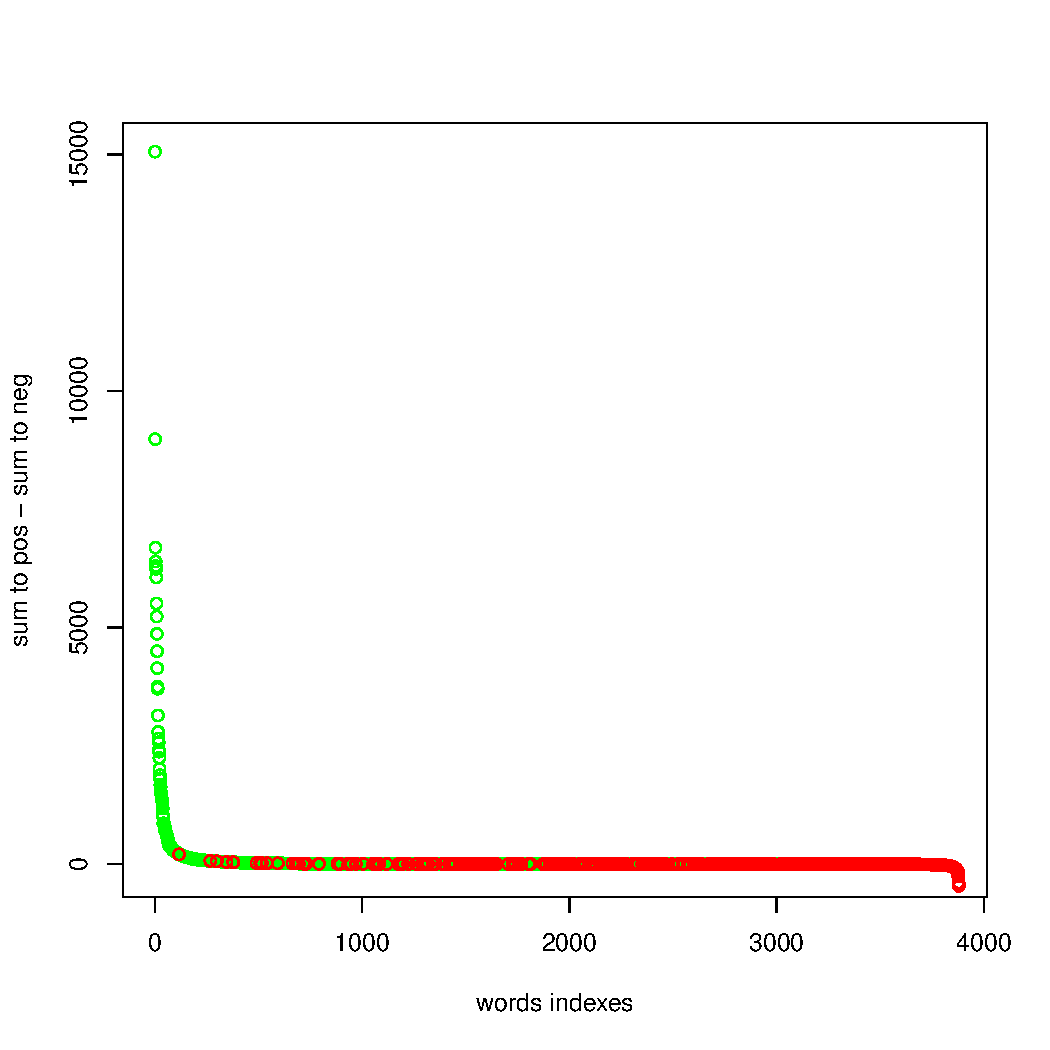
\includegraphics[width=\maxwidth]{figure/unnamed-chunk-71} 

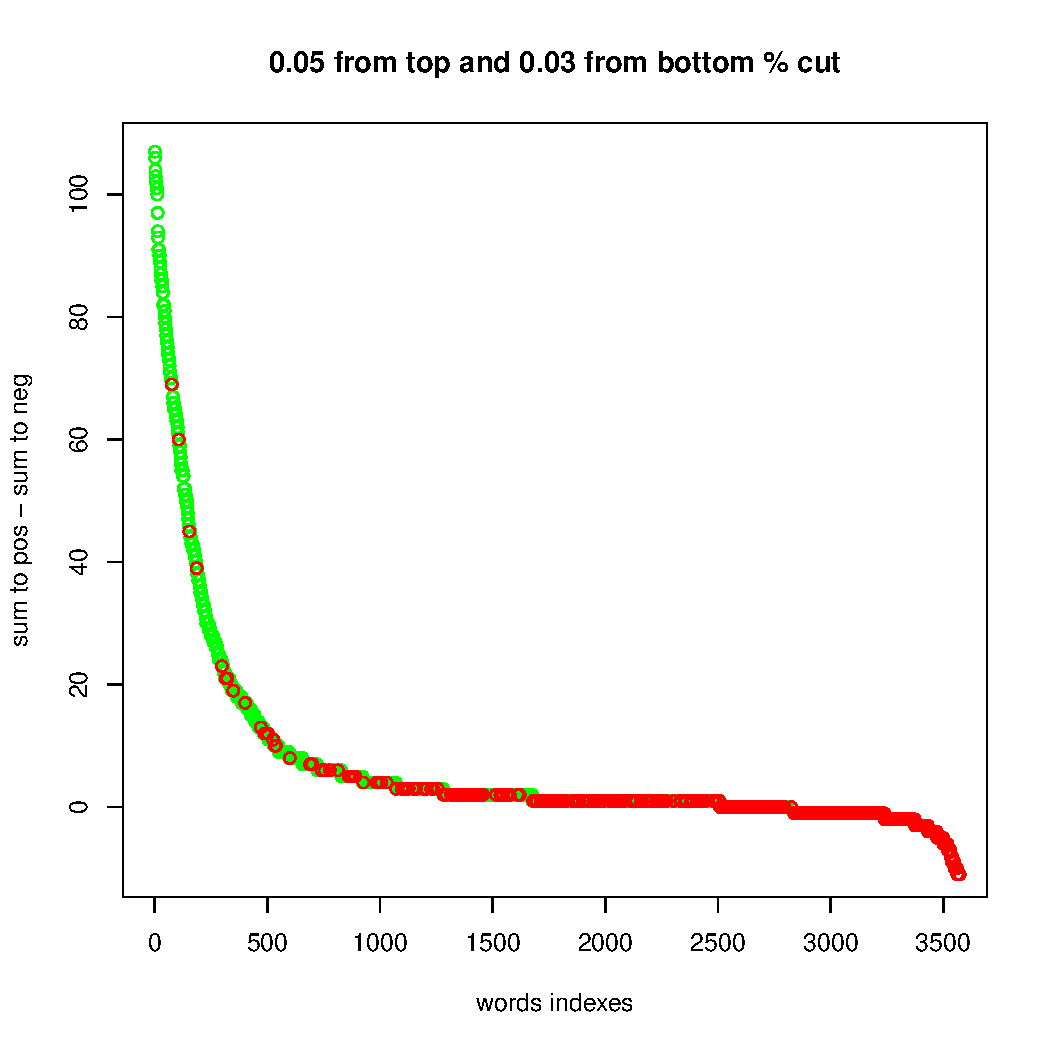
\includegraphics[width=\maxwidth]{figure/unnamed-chunk-72} 

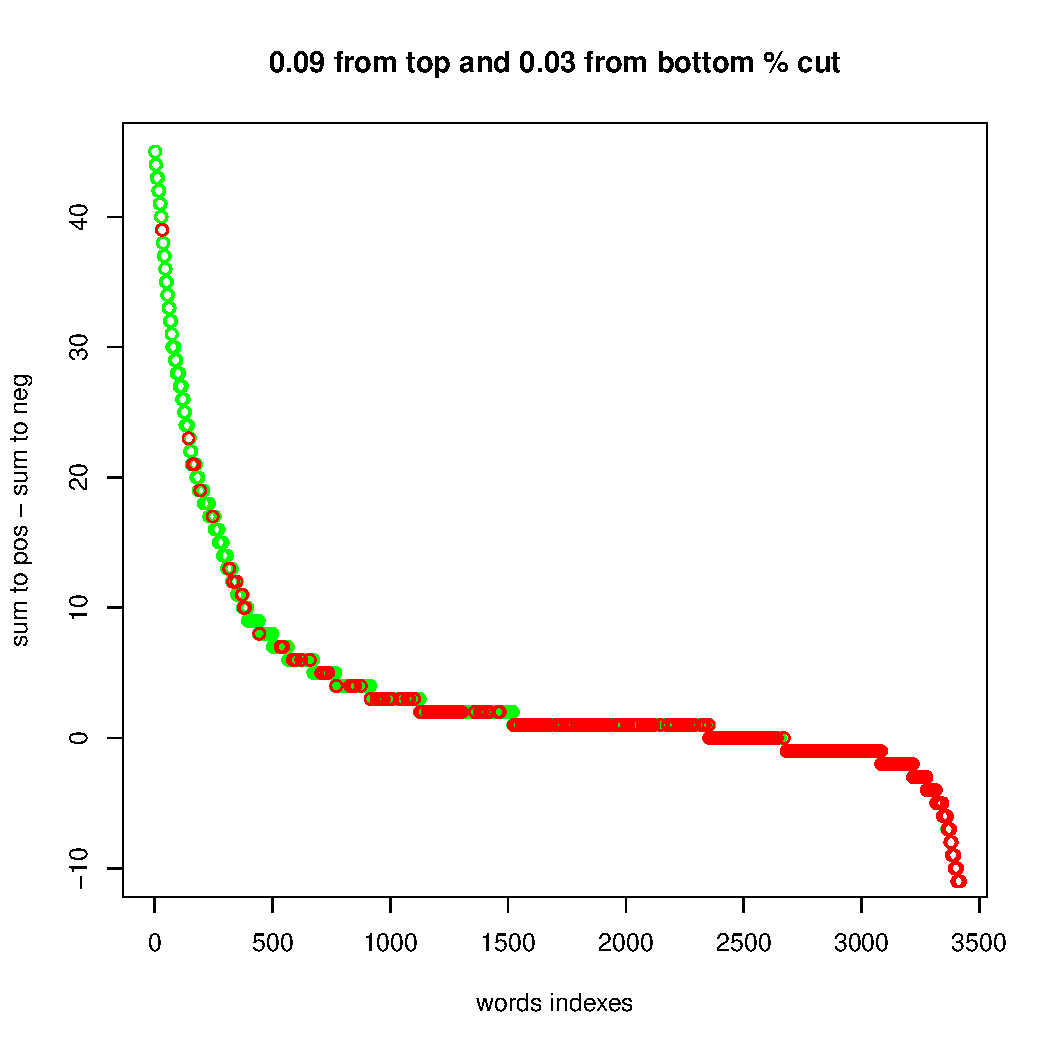
\includegraphics[width=\maxwidth]{figure/unnamed-chunk-73} 

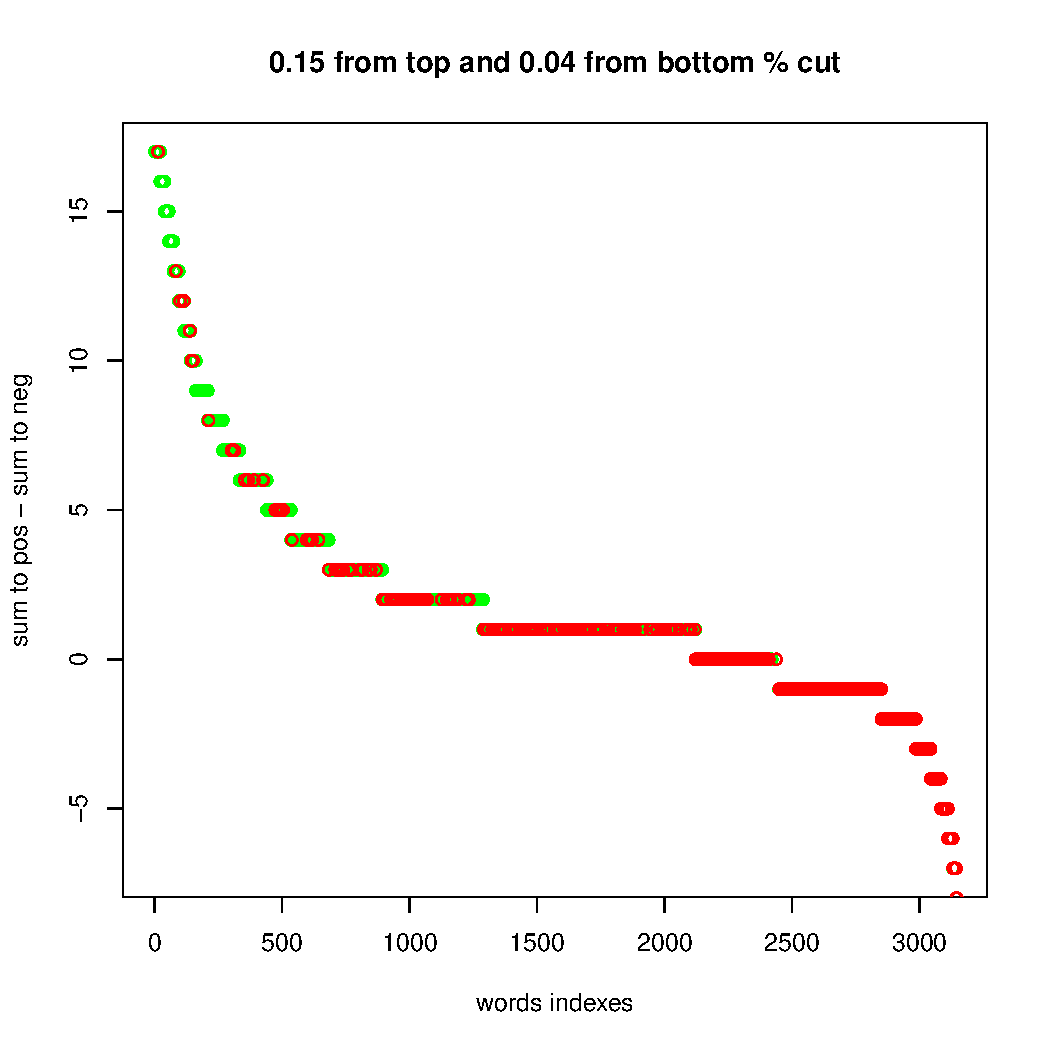
\includegraphics[width=\maxwidth]{figure/unnamed-chunk-74} 

\end{knitrout}


\begin{knitrout}
\definecolor{shadecolor}{rgb}{0.969, 0.969, 0.969}\color{fgcolor}
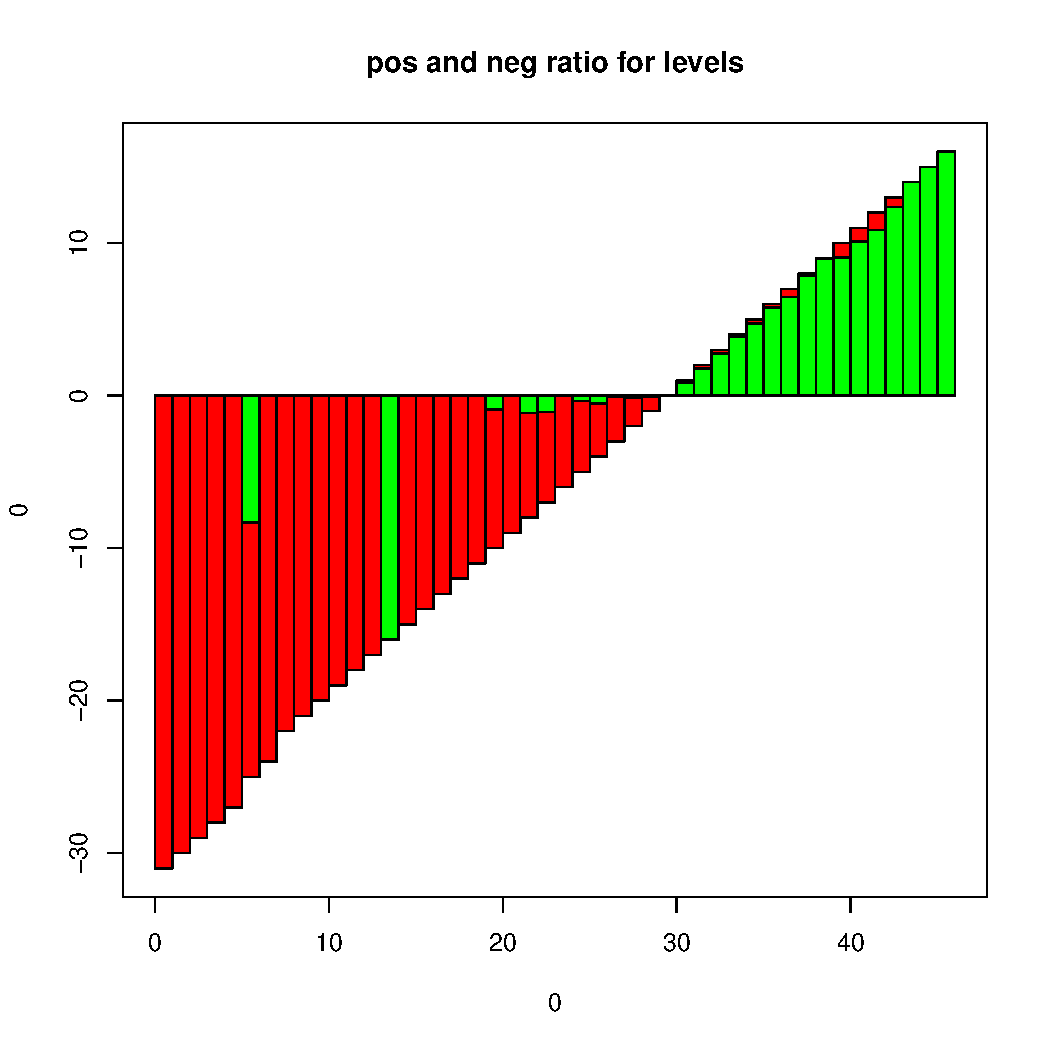
\includegraphics[width=\maxwidth]{figure/unnamed-chunk-8} 
\begin{kframe}\begin{verbatim}
## $lvl1
## [1] "-2"
## 
## $pos
##  [1] "бумажный"      "гниловатый"    "вальяжный"     "безжизненный"  "омерзительный"
##  [6] "дохлый"        "толстенький"   "захолустный"   "похабный"      "тощий"        
## 
## $neg
##   [1] "пустоватый"        "плохонький"        "курящий"           "напористый"       
##   [5] "бессовестный"      "куцый"             "избалованный"      "свежеокрашенный"  
##   [9] "грунтовый"         "безучастный"       "теологический"     "брезгливый"       
##  [13] "скотский"          "забывчивый"        "пассажирский"      "баварский"        
##  [17] "смехотворный"      "малокалорийный"    "напускной"         "видный"           
##  [21] "суровый"           "жутковатый"        "ведерный"          "малочисленный"    
##  [25] "вздорный"          "базарный"          "дряблый"           "банальный"        
##  [29] "изворотливый"      "портовый"          "аналогичный"       "абсурдный"        
##  [33] "сбивчивый"         "клинский"          "жидкий"            "волнистый"        
##  [37] "маниакальный"      "застоялый"         "наемный"           "плавучий"         
##  [41] "труднодоступный"   "полуголодный"      "купальный"         "коммунальный"     
##  [45] "битый"             "продолжительный"   "скупой"            "мелочный"         
##  [49] "никудышный"        "прошлогодний"      "безнадежный"       "хлорный"          
##  [53] "душещипательный"   "биохимический"     "аварийный"         "кованый"          
##  [57] "узенький"          "наркотический"     "бутафорский"       "издевательский"   
##  [61] "коренастый"        "костистый"         "крохотный"         "приторный"        
##  [65] "маломощный"        "сонный"            "кисловатый"        "свинцовый"        
##  [69] "жуликоватый"       "аховый"            "пожухлый"          "единообразный"    
##  [73] "жигулевский"       "вулканический"     "исключительный"    "слышный"          
##  [77] "обшарпанный"       "нудноватый"        "поганый"           "бугристый"        
##  [81] "отрывной"          "малокультурный"    "громкий"           "постижимый"       
##  [85] "вышеперечисленный" "невзрачный"        "апатичный"         "паршивый"         
##  [89] "заурядный"         "темненький"        "пастельный"        "проводной"        
##  [93] "слышимый"          "сельский"          "философский"       "фатальный"        
##  [97] "чумазый"           "червонный"         "пикантный"         "масенький"        
## [101] "кулинарный"        "трудоемкий"        "ниагарский"        "голенький"        
## [105] "шальной"           "пармский"          "оптовый"           "мстительный"      
## [109] "тривиальный"       "клейкий"           "юбилейный"         "обжитой"          
## [113] "эгоистичный"       "полненький"        "ничтожный"         "редкостный"       
## [117] "пузатенький"       "совершенный"       "хмелевой"          "удалый"           
## [121] "нестерпимый"       "цепкий"            "чартерный"         "злющий"           
## [125] "тепличный"        
## 
## $lvl1
## [1] "-1"
## 
## $pos
##  [1] "лицензионный"        "бдительный"          "речной"             
##  [4] "академичный"         "больничный"          "полый"              
##  [7] "минеральный"         "больной"             "слякотный"          
## [10] "здоровенный"         "плесневой"           "автодорожный"       
## [13] "водонепроницаемый"   "алтарный"            "досадный"           
## [16] "матерчатый"          "взыскательный"       "антисанитарный"     
## [19] "малопривлекательный" "вульгарный"          "хреновый"           
## [22] "самоуверенный"       "ангельский"          "тростниковый"       
## [25] "угловатый"           "трагичный"           "низкопробный"       
## 
## $neg
##   [1] "многословный"          "асфальтный"            "легонький"            
##   [4] "однополосный"          "бесснежный"            "зеленовато-синий"     
##   [7] "кишечный"              "округлый"              "возмутительный"       
##  [10] "волнозащитный"         "разводный"             "древнерусский"        
##  [13] "титанический"          "запрелый"              "заварочный"           
##  [16] "проблемный"            "вышеописанный"         "виновный"             
##  [19] "замужний"              "невежественный"        "проезжий"             
##  [22] "ходячий"               "связанный"             "зазорный"             
##  [25] "архаичный"             "катастрофический"      "односложный"          
##  [28] "убийственный"          "еженедельный"          "двуместный"           
##  [31] "выборочный"            "квелый"                "надрывный"            
##  [34] "маркий"                "кормовой"              "зловонный"            
##  [37] "критичный"             "безыскусный"           "изысканный"           
##  [40] "нахрапистый"           "барочный"              "зерненый"             
##  [43] "лихорадочный"          "должный"               "согласный"            
##  [46] "ветряный"              "драматичный"           "безвыходный"          
##  [49] "беззащитный"           "пресловутый"           "нефтеперерабатывающий"
##  [52] "жженый"                "нудистский"            "категоричный"         
##  [55] "зеленовато-желтый"     "второсортный"          "пользовательский"     
##  [58] "разборный"             "асфальтовый"           "дремучий"             
##  [61] "громогласный"          "летальный"             "ущербный"             
##  [64] "дефицитный"            "абразивный"            "пылеобразный"         
##  [67] "трудовой"              "босой"                 "радиоуправляемый"     
##  [70] "многотрудный"          "обыденный"             "длинненький"          
##  [73] "истребимый"            "аэрофлотовский"        "вменяемый"            
##  [76] "ключевой"              "давнишний"             "тяжкий"               
##  [79] "вольный"               "раритетный"            "остаточный"           
##  [82] "прижимистый"           "туговатый"             "горластый"            
##  [85] "дивноморский"          "белозубый"             "дюймовый"             
##  [88] "прибрежный"            "мускулистый"           "лысоватый"            
##  [91] "плиточный"             "гнусный"               "глупенький"           
##  [94] "дурной"                "тугой"                 "обледенелый"          
##  [97] "беспринципный"         "громкоговорящий"       "бессодержательный"    
## [100] "малоприятный"          "жилистый"              "предварительный"      
## [103] "малоразговорчивый"     "бесталанный"           "двуличный"            
## [106] "аляповатый"            "двухнедельный"         "приграничный"         
## [109] "односторонний"         "кондовый"              "глуповатый"           
## [112] "кустарный"             "беломраморный"         "малогабаритный"       
## [115] "гнусавый"              "делимый"               "легковой"             
## [118] "переменчивый"          "малый"                 "мышечный"             
## [121] "отставной"             "суетливый"             "лагерный"             
## [124] "запутанный"            "искусный"              "нарезной"             
## [127] "звукопроницаемый"      "кустистый"             "интуитивный"          
## [130] "премилый"              "сменный"               "береженый"            
## [133] "значительный"          "зоркий"                "туманный"             
## [136] "поганенький"           "пригорелый"            "бесчувственный"       
## [139] "инертный"              "возвратный"            "добровольный"         
## [142] "бездушный"             "дрянной"               "вообразимый"          
## [145] "многозначительный"     "тротуарный"            "дисковый"             
## [148] "ложный"                "лицеприятный"          "потребительский"      
## [151] "двусторонний"          "сбыточный"             "неупакованный"        
## [154] "обгорелый"             "расплывчатый"          "сатиновый"            
## [157] "комильфо"              "отвратимый"            "бесправный"           
## [160] "катастрофичный"        "растяжимый"            "икорный"              
## [163] "вкусовой"              "зябкий"                "венный"               
## [166] "неработающий"          "калининградский"       "презренный"           
## [169] "инфантильный"          "летучий"               "депрессивный"         
## [172] "декоративный"          "ватерпольный"          "максимальный"         
## [175] "инвалидный"            "отличимый"             "дураковатый"          
## [178] "малоприветливый"       "конфетный"             "высоковатый"          
## [181] "доморощенный"          "занятый"               "достижимый"           
## [184] "любвеобильный"         "галилейский"           "двусмысленный"        
## [187] "избитый"               "мой"                   "аскетический"         
## [190] "перманентный"          "горелый"               "законченный"          
## [193] "водительский"          "визитный"              "занудливый"           
## [196] "бюрократический"       "рыбацкий"              "высококалорийный"     
## [199] "вязкий"                "направленный"          "буржуйский"           
## [202] "долинный"              "добренький"            "треугольный"          
## [205] "виртуальный"           "плоховатый"            "заповедный"           
## [208] "голословный"           "колхозный"             "относительный"        
## [211] "крепенький"            "майонезный"            "бритоголовый"         
## [214] "давящий"               "феодальный"            "туристский"           
## [217] "утилитарный"           "халтурный"             "недоразвитый"         
## [220] "критический"           "ялтинский"             "половинчатый"         
## [223] "сухонький"             "шипучий"               "томительный"          
## [226] "кулуарный"             "формальный"            "комичный"             
## [229] "одинокий"              "тягостный"             "тревожный"            
## [232] "бессильный"            "показной"              "скуповатый"           
## [235] "судорожный"            "уморительный"          "удушливый"            
## [238] "эклектичный"           "однобокий"             "холуйский"            
## [241] "валлийский"            "прованский"            "пуританский"          
## [244] "малоговорящий"         "индифферентный"        "раскидистый"          
## [247] "регулируемый"          "лилипутский"           "идентичный"           
## [250] "минималистический"     "заштатный"             "суеверный"            
## [253] "летный"                "исправимый"            "полукруглый"          
## [256] "поправимый"            "травматичный"          "плохенький"           
## [259] "срочный"               "переполненный"         "сопливый"             
## [262] "нищий"                 "замшелый"              "отталкивающий"        
## [265] "шумливый"              "плаксивый"             "тупорылый"            
## [268] "членный"               "стручковый"            "морщинистый"          
## [271] "фактический"           "масленый"              "лоточный"             
## [274] "щупленький"            "толстопузый"           "носастый"             
## [277] "пузырчатый"            "июньский"              "чахлый"               
## [280] "первоочередный"        "раненый"               "пастообразный"        
## [283] "уловимый"              "сальный"               "сейшельский"          
## [286] "учебный"               "леопардовый"           "нашенский"            
## [289] "меркантильный"         "охочий"                "сермяжный"            
## [292] "процедурный"           "мыслимый"              "труднодостижимый"     
## [295] "хельсинкский"          "снобистский"           "спесивый"             
## [298] "малообразованный"      "марсовый"              "цокольный"            
## [301] "красноватый"           "тепловатый"            "настырный"            
## [304] "узорчатый"             "утоптанный"            "скифский"             
## [307] "мафиозный"             "мереный"               "напряженный"          
## [310] "распущенный"           "неотъемлемый"          "рядовой"              
## [313] "ношеный"               "мажорный"              "отсталый"             
## [316] "чудодейственный"       "роковый"               "пластилиновый"        
## [319] "клеклый"               "однокомпонентный"      "дежурный"             
## [322] "трухлявый"             "экстренный"            "цементный"            
## [325] "клинический"           "серо-синий"            "многочасовой"         
## [328] "ненавистный"           "сквозной"              "сведущий"             
## [331] "полиэтиленовый"        "травянистый"           "сиротливый"           
## [334] "скверный"              "ископаемый"            "чрезвычайный"         
## [337] "чердачный"             "похотливый"            "истеричный"           
## [340] "инородный"             "марсианский"           "купейный"             
## [343] "циничный"              "промысловый"           "употребимый"          
## [346] "штучный"               "электронно-лучевой"    "тряпичный"            
## [349] "черноватый"            "однослойный"           "чернявенький"         
## [352] "щуплый"                "прискорбный"           "проницаемый"          
## [355] "железобетонный"        "реликтовый"            "уродский"             
## [358] "побочный"              "цикличный"             "раздаточный"          
## [361] "комковатый"            "престарелый"           "шкодливый"            
## [364] "майский"               "рукотворный"           "фривольный"           
## [367] "насильственный"        "сварливый"             "усидчивый"            
## [370] "соблазнительный"       "необузданный"          "фермерский"           
## [373] "пунцовый"              "худющий"               "слаборазвитый"        
## 
## $lvl1
## [1] "0"
## 
## $pos
##  [1] "решительный"            "звонкий"                "разнокалиберный"       
##  [4] "беспорядочный"          "разбитной"              "педантичный"           
##  [7] "импульсивный"           "беспощадный"            "заядлый"               
## [10] "проникновенный"         "слоистый"               "многодетный"           
## [13] "патриархальный"         "мыльный"                "беспомощный"           
## [16] "выигрышный"             "канатный"               "колючий"               
## [19] "очный"                  "вафельный"              "безразмерный"          
## [22] "лютый"                  "добросердечный"         "малоподвижный"         
## [25] "газовый"                "изможденный"            "образный"              
## [28] "низенький"              "грузовой"               "пупырчатый"            
## [31] "механический"           "неподготовленный"       "лицемерный"            
## [34] "развязный"              "расчетливый"            "пронырливый"           
## [37] "душераздирающий"        "вездесущий"             "невыносимый"           
## [40] "педальный"              "нескончаемый"           "культурно-исторический"
## [43] "праздный"               "корыстный"              "смотровой"             
## [46] "живительный"            "картонный"              "мертвый"               
## [49] "дерьмовый"              "свинский"               "высокотемпературный"   
## [52] "самодовольный"          "самодеятельный"         "чудовищный"            
## [55] "шаблонный"              "прощальный"             "тихенький"             
## [58] "цыганский"              "труднопроходимый"       "полудетский"           
## [61] "ухабистый"              "тинный"                 "темно-серый"           
## [64] "разноголосый"           "равный"                 "скальный"              
## [67] "рослый"                 "трехкомнатный"          "копеечный"             
## [70] "осклизлый"              "смородиновый"           "придорожный"           
## [73] "мнительный"             "хлористый"              "слащавый"              
## [76] "уксусный"               "своенравный"           
## 
## $neg
##  [1] "редкий"               "заключительный"       "желательный"         
##  [4] "покупной"             "беспредельный"        "трехъярусный"        
##  [7] "обветшалый"           "пожилой"              "электрический"       
## [10] "привязчивый"          "круговой"             "задумчивый"          
## [13] "коротенький"          "марочный"             "индустриальный"      
## [16] "гениальный"           "бессистемный"         "непредвиденный"      
## [19] "костлявый"            "возрастной"           "казенный"            
## [22] "варварский"           "обеспеченный"         "очевидный"           
## [25] "понтонный"            "водоплавающий"        "рейсовый"            
## [28] "дотошный"             "лысенький"            "волнительный"        
## [31] "трехразовый"          "страшноватый"         "пахучий"             
## [34] "запретный"            "допустимый"           "порочный"            
## [37] "сероватый"            "надземный"            "жирноватый"          
## [40] "дешевенький"          "запредельный"         "привозный"           
## [43] "преодолимый"          "земной"               "самовлюбленный"      
## [46] "затрапезный"          "малозаметный"         "легальный"           
## [49] "движимый"             "истинный"             "ординарный"          
## [52] "заоблачный"           "ракушечный"           "изменчивый"          
## [55] "неизбежный"           "малоэффективный"      "безликий"            
## [58] "подозрительный"       "коротконогий"         "резиновый"           
## [61] "настенный"            "малоинформативный"    "однородный"          
## [64] "склонный"             "вводный"              "плотненький"         
## [67] "оправданный"          "преклонный"           "рыжий"               
## [70] "цензурный"            "системный"            "хилый"               
## [73] "явный"                "штопаный"             "полуподвальный"      
## [76] "приморский"           "типовой"              "флегматичный"        
## [79] "устранимый"           "уверенный"            "транзитный"          
## [82] "полноватый"           "сельскохозяйственный" "часовой"             
## [85] "трусливый"            "худенький"            "младенческий"        
## [88] "рубленый"             "совместимый"          "простецкий"          
## [91] "экстраординарный"     "серный"               "стальной"            
## [94] "эксцентричный"        "холостой"             "махонький"           
## [97] "стратегический"       "центровой"            "прожорливый"         
## 
## $lvl1
## [1] "1"
## 
## $pos
##   [1] "бурый"                "знойный"              "песенный"            
##   [4] "дородный"             "парикмахерский"       "затхлый"             
##   [7] "толстощекий"          "полуоткрытый"         "богохульный"         
##  [10] "посольский"           "паршивенький"         "полосный"            
##  [13] "индусский"            "лопоухий"             "масленичный"         
##  [16] "адмиральский"         "алкоголический"       "въедливый"           
##  [19] "гимнастический"       "заменимый"            "карточный"           
##  [22] "гладильный"           "восточно-азиатский"   "пропорциональный"    
##  [25] "бесперебойный"        "зефирный"             "занозистый"          
##  [28] "низменный"            "целеустремленный"     "полуторачасовой"     
##  [31] "певучий"              "прицепной"            "иноземный"           
##  [34] "авторский"            "реденький"            "соборный"            
##  [37] "артиллерийский"       "сопоставимый"         "отлогий"             
##  [40] "льготный"             "жидкокристаллический" "безыдейный"          
##  [43] "взлетный"             "перпендикулярный"     "гражданский"         
##  [46] "трехцветный"          "безрадостный"         "библейский"          
##  [49] "равнинный"            "врезной"              "рачительный"         
##  [52] "банковый"             "задушевный"           "почетный"            
##  [55] "сенсорный"            "точечный"             "длинноногий"         
##  [58] "зримый"               "азербайджанский"      "семиэтажный"         
##  [61] "документальный"       "плавленый"            "крестьянский"        
##  [64] "первоначальный"       "дообеденный"          "аптечный"            
##  [67] "вспыльчивый"          "общедоступный"        "мускатный"           
##  [70] "кардный"              "полупустынный"        "манерный"            
##  [73] "амбарный"             "кровный"              "океанский"           
##  [76] "джентльменский"       "кряжистый"            "бальнеологический"   
##  [79] "одновременный"        "высокопоставленный"   "желеобразный"        
##  [82] "демисезонный"         "затяжной"             "лигурийский"         
##  [85] "дальновидный"         "лилово-синий"         "лукавый"             
##  [88] "ломаный"              "реечный"              "рыболовный"          
##  [91] "пурпурный"            "бревенчатый"          "великоморавский"     
##  [94] "трехдневный"          "бассейный"            "закусочный"          
##  [97] "пошловатый"           "недобитый"            "многократный"        
## [100] "билетный"             "благонадежный"        "ежевечерний"         
## [103] "белокурый"            "ходкий"               "глубоководный"       
## [106] "адыгейский"           "магнитный"            "ангарный"            
## [109] "насосный"             "лиричный"             "пасмурный"           
## [112] "выносливый"           "гарный"               "барселонский"        
## [115] "новомодный"           "молекулярный"         "симметричный"        
## [118] "видовой"              "корпусный"            "многоплановый"       
## [121] "лощеный"              "подветренный"         "непонятый"           
## [124] "образовательный"      "горяченький"          "винодельческий"      
## [127] "дымчатый"             "барбадосский"         "неприкрытый"         
## [130] "индейский"            "горчичный"            "алычовый"            
## [133] "вопиющий"             "карикатурный"         "патетичный"          
## [136] "вакуумный"            "загробный"            "беззубый"            
## [139] "глуховатый"           "панибратский"         "бессменный"          
## [142] "иорданский"           "волосатенький"        "косячный"            
## [145] "имущественный"        "бродильный"           "взаимозаменяемый"    
## [148] "меткий"               "бамбуковый"           "насущный"            
## [151] "комический"           "предрождественский"   "бездумный"           
## [154] "отделочный"           "красно-коричневый"    "психический"         
## [157] "маточный"             "горший"               "оманский"            
## [160] "москитный"            "агитационный"         "податливый"          
## [163] "периферический"       "архимандритский"      "безмерный"           
## [166] "дворянский"           "диабетический"        "аппаратный"          
## [169] "интригующий"          "расовый"              "академический"       
## [172] "зигзагообразный"      "безумный"             "процентный"          
## [175] "влюбчивый"            "боязливый"            "паразитический"      
## [178] "стилистический"       "пятерочный"           "жирненький"          
## [181] "беззлобный"           "полупьяный"           "сумрачный"           
## [184] "еловый"               "бальзамический"       "междугородний"       
## [187] "канализационный"      "практический"         "вокальный"           
## [190] "бестелесный"          "безболезненный"       "магнетический"       
## [193] "жиденький"            "импозантный"          "головастый"          
## [196] "бессрочный"           "костный"              "методичный"          
## [199] "квашеный"             "безосновательный"     "кафедральный"        
## [202] "живучий"              "длиннющий"            "безапелляционный"    
## [205] "звуконепроницаемый"   "афганский"            "жестяной"            
## [208] "посторонний"          "анчоусный"            "несказанный"         
## [211] "легкоатлетический"    "багровый"             "многоязычный"        
## [214] "напольный"            "благорасположенный"   "изначальный"         
## [217] "потенциальный"        "здравый"              "продовольственный"   
## [220] "фамильярный"          "ноу"                  "акробатический"      
## [223] "вихревой"             "сторожевой"           "блистательный"       
## [226] "дьявольский"          "освежающий"           "вертлявый"           
## [229] "многовариантный"      "краткосрочный"        "довоенный"           
## [232] "давленый"             "головной"             "седовласый"          
## [235] "призрачный"           "бело-розовый"         "общечеловеческий"    
## [238] "брутальный"           "антарктический"       "кнопочный"           
## [241] "сверхновый"           "кроликовый"           "бездонный"           
## [244] "плавательный"         "алтайский"            "мужиковатый"         
## [247] "возвышенный"          "приближенный"         "оглушительный"       
## [250] "фронтовой"            "ковбойский"           "конкурсный"          
## [253] "китийский"            "примерный"            "пружинистый"         
## [256] "меланхоличный"        "неукоснительный"      "боярский"            
## [259] "монопольный"          "погожий"              "грузный"             
## [262] "двухразовый"          "ольгинский"           "концертный"          
## [265] "минутный"             "коста-риканский"      "целебный"            
## [268] "малообщительный"      "безукоризненный"      "суточный"            
## [271] "заработный"           "донецкий"             "сердитый"            
## [274] "предпочтительный"     "здравомыслящий"       "диагностический"     
## [277] "безнаказанный"        "политический"         "осторожный"          
## [280] "кучерявый"            "болотный"             "аборигенский"        
## [283] "обстоятельный"        "образцовый"           "западноевропейский"  
## [286] "рефлексный"           "многолетний"          "враждебный"          
## [289] "литровый"             "коробочный"           "великодушный"        
## [292] "артезианский"         "оконный"              "витиеватый"          
## [295] "заунывный"            "дамский"              "аномальный"          
## [298] "малопригодный"        "большегрузный"        "арочный"             
## [301] "покладистый"          "ассоциативный"        "греховный"           
## [304] "вересковый"           "поведенческий"        "ворсистый"           
## [307] "ливерный"             "бесславный"           "гурьевский"          
## [310] "годный"               "высокопарный"         "ламповый"            
## [313] "дореволюционный"      "отвесный"             "рождественский"      
## [316] "аравийский"           "балаганный"           "каминный"            
## [319] "позапрошлый"          "материковый"          "всемирный"           
## [322] "зубоврачебный"        "жестокий"             "геронтологический"   
## [325] "поселковый"           "гранитный"            "социологический"     
## [328] "буковый"              "дегустационный"       "алый"                
## [331] "ливневый"             "организационный"      "сутулый"             
## [334] "глубинный"            "военный"              "благовоспитанный"    
## [337] "пробочный"            "красноречивый"        "воспитательный"      
## [340] "амебный"              "свойский"             "малайзийский"        
## [343] "безголосый"           "штильный"             "защитный"            
## [346] "порожняковый"         "татарский"            "покойный"            
## [349] "безотходный"          "опереточный"          "взрывной"            
## [352] "наблюдательный"       "антистрессовый"       "будапештский"        
## [355] "арнаутский"           "символичный"          "кусковой"            
## [358] "океанический"         "сумочный"             "приоритетный"        
## [361] "сборный"              "низкотемпературный"   "институтский"        
## [364] "засушливый"           "подпорный"            "диковинный"          
## [367] "велюровый"            "богемный"             "рекреационный"       
## [370] "женственный"          "двадцатилетний"       "макаронный"          
## [373] "выносной"             "большеносый"          "всепрощающий"        
## [376] "вышеуказанный"        "винтообразный"        "боковой"             
## [379] "периодичный"          "призматический"       "вербеновый"          
## [382] "бассейновый"          "фольклорный"          "скептический"        
## [385] "земляничный"          "иконный"              "бесстрашный"         
## [388] "фактурный"            "тошнотворный"         "южноамериканский"    
## [391] "хвастливый"           "русоволосый"          "футуристический"     
## [394] "пухлый"               "дурашливый"           "прогрессивный"       
## [397] "охристый"             "пористый"             "начальный"           
## [400] "ошеломительный"       "тщеславный"           "непроизносимый"      
## [403] "чугунный"             "чумовой"              "шкурный"             
## [406] "трехзвездочный"       "статусный"            "страховой"           
## [409] "схематичный"          "шестиэтажный"         "сиамский"            
## [412] "пленительный"         "неопознанный"         "повторный"           
## [415] "беспрепятственный"    "лимитный"             "терский"             
## [418] "скрупулезный"         "развесистый"          "уездный"             
## [421] "проездной"            "секретный"            "закономерный"        
## [424] "сине-зеленый"         "сегодняшний"          "поэтический"         
## [427] "повальный"            "фундаментальный"      "карнавальный"        
## [430] "сладкоголосый"        "пионерский"           "русофобский"         
## [433] "эмиграционный"        "невиданный"           "подлинный"           
## [436] "сакральный"           "читальный"            "свежевыбритый"       
## [439] "целенький"            "смирный"              "сигаретный"          
## [442] "пылкий"               "преогромный"          "компромиссный"       
## [445] "придурковатый"        "скорбный"             "толстенный"          
## [448] "темно-коричневый"     "изразцовый"           "утлый"               
## [451] "скульптурный"         "хоккейный"            "овальный"            
## [454] "ярко-фиолетовый"      "продувной"            "кроткий"             
## [457] "оборотистый"          "этичный"              "шри-ланкийский"      
## [460] "римский"              "таллинский"           "охотный"             
## [463] "резковатый"           "криволинейный"        "увесистый"           
## [466] "монолитный"           "сверхъестественный"   "многорукий"          
## [469] "флорентийский"        "ругательный"          "зональный"           
## [472] "репрезентативный"     "трехстворчатый"       "мартовский"          
## [475] "розоватый"            "толченый"             "сырокопченый"        
## [478] "духовой"              "свежевыкрашенный"     "страстный"           
## [481] "литейный"             "обольстительный"      "отважный"            
## [484] "дымный"               "союзный"              "многострадальный"    
## [487] "трехслойный"          "целомудренный"        "разрушительный"      
## [490] "пересадочный"         "розмариновый"         "фабричный"           
## [493] "непомерный"           "общенациональный"     "колумбийский"        
## [496] "морошковый"           "склочный"             "эгоцентричный"       
## [499] "водопадный"           "лихой"                "тотальный"           
## [502] "верткий"              "створчатый"           "столетний"           
## [505] "минималистский"       "беспошлинный"         "пародийный"          
## [508] "цилиндрический"       "тогдашний"            "социалистический"    
## [511] "светлокожий"          "новозеландский"       "сокрушительный"      
## [514] "прокатный"            "обходный"             "худосочный"          
## [517] "публичный"            "кузнечный"            "стеклодувный"        
## [520] "промежуточный"        "хрусткий"             "фигуристый"          
## [523] "шашлычный"            "папирусовый"          "коммуникативный"     
## [526] "недурственный"        "рекламный"            "сдвижной"            
## [529] "назидательный"        "типажный"             "курьезный"           
## [532] "парашютный"           "трескучий"            "горочный"            
## [535] "микроволновый"        "мимолетный"           "древнеегипетский"    
## [538] "ситцевый"             "передний"             "ширпотребный"        
## [541] "платяной"             "закарпатский"         "токийский"           
## [544] "темно-желтый"         "темно-голубой"        "раннехристианский"   
## [547] "ярко-оранжевый"       "холеный"              "общепризнанный"      
## [550] "словарный"            "мальтийский"          "язычный"             
## [553] "фиджийский"           "хмуроватый"           "тюркоязычный"        
## [556] "многокрасочный"       "шутливый"             "республиканский"     
## [559] "ужинный"              "рогатый"              "минойский"           
## [562] "шустренький"          "рискованный"          "петроградский"       
## [565] "коньячный"            "тюркский"             "паштетный"           
## [568] "ячменный"             "мерзлый"              "лаковый"             
## [571] "подпольный"           "ленный"               "ришельевский"        
## [574] "ханойский"            "омский"               "федеральный"         
## [577] "никитский"            "рефлексивный"         "шланговый"           
## [580] "малосодержательный"   "норковый"             "малоприбыльный"      
## [583] "крученый"             "объездной"            "францисканский"      
## [586] "спиральный"           "товарный"             "титановый"           
## [589] "шлюпочный"            "прагматичный"         "тминный"             
## [592] "трафальгарский"       "ростовский"           "свежеотжатый"        
## [595] "зелено-желтый"        "непроглядный"         "мушкетерский"        
## [598] "терпковатый"          "поджелудочный"        "пасхальный"          
## [601] "прохладительный"      "доспелый"             "полновесный"         
## [604] "малоалкогольный"      "негритянский"         "норманнский"         
## [607] "чудненький"           "притворный"           "эфемерный"           
## [610] "ильный"               "ультрамодный"         "талый"               
## [613] "элитарный"            "краковский"           "секционный"          
## [616] "шенгенский"           "эротический"          "рязанский"           
## [619] "столичный"            "осветительный"        "свежезаваренный"     
## [622] "мандаринный"          "подставной"           "сухенький"           
## [625] "нижегородский"        "щенный"               "юмористический"      
## [628] "идиллический"         "супружеский"          "хвалебный"           
## [631] "уступчивый"           "угодливый"            "медный"              
## [634] "священный"            "порожистый"           "забористый"          
## [637] "неустанный"           "разухабистый"         "прибыльный"          
## [640] "легкомысленный"       "свежевымытый"         "злачный"             
## [643] "читабельный"          "крабовый"             "региональный"        
## [646] "хозяйский"            "перловый"             "непереводимый"       
## [649] "картографический"     "фоновый"              "хипповый"            
## [652] "падуанский"           "яванский"             "энергетический"      
## [655] "мордатый"             "тощенький"            "целенаправленный"    
## [658] "утвердительный"       "перьевой"             "жалобный"            
## [661] "наборный"             "обонятельный"         "щавелевый"           
## [664] "послезавтрашний"      "топленый"             "укропный"            
## [667] "умилительный"         "фрагментарный"        "кипарисный"          
## [670] "шутейный"             "любовный"             "грантовый"           
## [673] "новочеркасский"       "онежский"             "кровопролитный"      
## [676] "представительский"    "полнотелый"           "капиталистический"   
## [679] "сходный"              "профильный"           "потрясающий"         
## [682] "яхтенный"             "потайной"             "статичный"           
## [685] "упоительный"          "топовый"              "фотогеничный"        
## [688] "соответственный"      "непобедимый"          "мелкодонный"         
## [691] "волновой"             "нескрываемый"         "одноименный"         
## [694] "ладненький"           "помойный"             "топорный"            
## [697] "низкосортный"         "опальный"             "малосольный"         
## [700] "куполообразный"       "слизкий"              "юродивый"            
## [703] "южнокитайский"        "виртуозный"           "старочешский"        
## [706] "рассветный"           "храбрый"              "розовенький"         
## [709] "сексапильный"         "угарный"              "независящий"         
## [712] "цепной"               "полицейский"          "режиссерский"        
## [715] "маслодельный"         "логический"           "серо-голубой"        
## [718] "шкатулочный"          "упрямый"              "утопический"         
## [721] "унывный"              "перепрелый"           "прелый"              
## [724] "новгородский"         "ушной"                "пестренький"         
## [727] "копровый"            
## 
## $neg
##   [1] "мифический"          "забойный"            "доисторический"     
##   [4] "выполнимый"          "бордовый"            "альтернативный"     
##   [7] "левосторонний"       "непролазный"         "обрывчатый"         
##  [10] "малограмотный"       "безусловный"         "долговечный"        
##  [13] "влагостойкий"        "мощеный"             "нелетающий"         
##  [16] "безызвестный"        "наивный"             "несуразный"         
##  [19] "изгибистый"          "бочковый"            "схожий"             
##  [22] "жестковатый"         "биометрический"      "благостный"         
##  [25] "миловидный"          "водяной"             "закомплексованный"  
##  [28] "доверчивый"          "клеточный"           "высотный"           
##  [31] "венский"             "нарочитый"           "круглолицый"        
##  [34] "дохленький"          "моравский"           "рыхлый"             
##  [37] "стеснительный"       "бетонный"            "финансовый"         
##  [40] "черноморский"        "дорогостоящий"       "бензиновый"         
##  [43] "излишний"            "моментальный"        "буддистский"        
##  [46] "однократный"         "каскадный"           "планомерный"        
##  [49] "бронзовый"           "непоседливый"        "догадливый"         
##  [52] "заспанный"           "бритый"              "питерский"          
##  [55] "рифленый"            "бесстыдный"          "свойственный"       
##  [58] "хлипкий"             "светло-серый"        "ведомственный"      
##  [61] "скользкий"           "именитый"            "характерный"        
##  [64] "жухлый"              "разительный"         "четырехзвездочный"  
##  [67] "иллюзорный"          "темноволосый"        "охраняемый"         
##  [70] "тихонький"           "тирренский"          "уклюжий"            
##  [73] "табачный"            "ярусный"             "прозорливый"        
##  [76] "спутниковый"         "проходимый"          "тухловатый"         
##  [79] "демократический"     "серо-буро-малиновый" "парадоксальный"     
##  [82] "стопроцентный"       "подвесной"           "поддельный"         
##  [85] "щепетильный"         "парниковый"          "светский"           
##  [88] "праведный"           "одиозный"            "релаксационный"     
##  [91] "сдельный"            "досрочный"           "этический"          
##  [94] "чанный"              "тамошний"            "сингальский"        
##  [97] "крупногабаритный"    "сдержанный"          "оборонительный"     
## [100] "славненький"         "сбалансированный"    "сменяемый"          
## [103] "умеренный"           "развитый"            "умозрительный"      
## [106] "ужасающий"          
## 
## $lvl1
## [1] "2"
## 
## $pos
##   [1] "полутемный"          "отчетливый"          "коммерческий"       
##   [4] "древнеримский"       "листовой"            "символический"      
##   [7] "случайный"           "коечный"             "искрометный"        
##  [10] "многоцветный"        "кипяченый"           "мозаичный"          
##  [13] "малосоленый"         "гнилостный"          "пристальный"        
##  [16] "многовековой"        "низкорослый"         "гавайский"          
##  [19] "мясистый"            "недвижный"           "неимоверный"        
##  [22] "нагой"               "ответный"            "краснокочанный"     
##  [25] "вариантный"          "дачный"              "хаотичный"          
##  [28] "организаторский"     "теперешний"          "тыльный"            
##  [31] "голосистый"          "реалистичный"        "салатный"           
##  [34] "екатеринбургский"    "героический"         "годовалый"          
##  [37] "подмосковный"        "нефтяной"            "джазовый"           
##  [40] "льняной"             "латвийский"          "мизерный"           
##  [43] "васильковый"         "пригожий"            "ориентированный"    
##  [46] "деятельный"          "абхазский"           "медитативный"       
##  [49] "авиационный"         "симфонический"       "описательный"       
##  [52] "писклявый"           "игристый"            "калифорнийский"     
##  [55] "атласский"           "албанский"           "сотовый"            
##  [58] "бессмертный"         "избыточный"          "доверительный"      
##  [61] "аленький"            "загородный"          "всепоглощающий"     
##  [64] "сострадательный"     "всепроникающий"      "подъездный"         
##  [67] "идиотский"           "межэтнический"       "курчавый"           
##  [70] "горнолыжный"         "сокровенный"         "беспокойный"        
##  [73] "правосторонний"      "балтийский"          "рельефный"          
##  [76] "башкирский"          "комедийный"          "давний"             
##  [79] "великобританский"    "носатый"             "крутоватый"         
##  [82] "многоразовый"        "малонаселенный"      "размерный"          
##  [85] "каучуковый"          "амбициозный"         "творческий"         
##  [88] "продуктивный"        "молниеносный"        "беспрерывный"       
##  [91] "ремесленный"         "авторитетный"        "невозмутимый"       
##  [94] "потешный"            "дугообразный"        "идейный"            
##  [97] "протяжный"           "приветный"           "выдержанный"        
## [100] "лубочный"            "зыбкий"              "производственный"   
## [103] "пригородный"         "сивый"               "однокамерный"       
## [106] "белесый"             "гладкошерстный"      "бесспорный"         
## [109] "лучистый"            "бактерицидный"       "благообразный"      
## [112] "высококачественный"  "латышский"           "бурятский"          
## [115] "законопослушный"     "агентский"           "безмолвный"         
## [118] "родниковый"          "трансформаторный"    "едкий"              
## [121] "детальный"           "иранский"            "светло-зеленый"     
## [124] "полусонный"          "кикладский"          "сандаловый"         
## [127] "кудрявый"            "звуковой"            "адреналиновый"      
## [130] "суздальский"         "ступенчатый"         "принципиальный"     
## [133] "въездной"            "ротанговый"          "смазливый"          
## [136] "автономный"          "многокилометровый"   "мануальный"         
## [139] "парламентский"       "кастовый"            "желто-зеленый"      
## [142] "обетованный"         "свиной"              "бесконтрольный"     
## [145] "быстрорастворимый"   "крепковатый"         "многоголосый"       
## [148] "единичный"           "воскресный"          "докторский"         
## [151] "соревновательный"    "изобретательный"     "кризисный"          
## [154] "беспосадочный"       "драконовый"          "зловещий"           
## [157] "безудержный"         "печальный"           "долгосрочный"       
## [160] "иерусалимский"       "ближневосточный"     "багажный"           
## [163] "высокооплачиваемый"  "ослепительный"       "тунцовый"           
## [166] "паломнический"       "паленый"             "концептуальный"     
## [169] "визуальный"          "каштановый"          "хлопковый"          
## [172] "недозревший"         "коричневатый"        "козырный"           
## [175] "своевольный"         "проливной"           "зубастый"           
## [178] "повсеместный"        "косметологический"   "кисло-сладкий"      
## [181] "китовый"             "безымянный"          "лунный"             
## [184] "исламский"           "коротковатый"        "студенческий"       
## [187] "безмоторный"         "братский"            "высокоразвитый"     
## [190] "заблаговременный"    "бесценный"           "бесстрастный"       
## [193] "ортопедический"      "крепленый"           "безоглядный"        
## [196] "гостевой"            "бардовый"            "зрительный"         
## [199] "пуховый"             "завтрашний"          "кошеный"            
## [202] "абстрактный"         "белобрысый"          "нью-йоркский"       
## [205] "заграничный"         "кленовый"            "калужский"          
## [208] "бешеный"             "непромокаемый"       "многослойный"       
## [211] "броуновский"         "грудной"             "вдохновенный"       
## [214] "кабельный"           "базовый"             "благонравный"       
## [217] "пробивной"           "желейный"            "хваленый"           
## [220] "месячный"            "заплесневелый"       "корпоративный"      
## [223] "патлатый"            "мучной"              "преотличный"        
## [226] "близлежащий"         "однотонный"          "октябрьский"        
## [229] "закатный"            "проницательный"      "неоновый"           
## [232] "приземистый"         "кондитерский"        "пребольшой"         
## [235] "львиный"             "мусорный"            "дрожжевой"          
## [238] "круглогодичный"      "постановочный"       "винодельный"        
## [241] "расчудесный"         "сидячий"             "швейный"            
## [244] "кривоватый"          "палевый"             "равнозначный"       
## [247] "авангардистский"     "зубной"              "спаржевый"          
## [250] "чувствительный"      "эллинский"           "смолистый"          
## [253] "сорокалетний"        "асимметричный"       "трудноустранимый"   
## [256] "югославский"         "разноликий"          "цветастый"          
## [259] "щербатый"            "северо-западный"     "юго-западный"       
## [262] "умственный"          "юго-восточный"       "этрусский"          
## [265] "последующий"         "церковный"           "хлебосольный"       
## [268] "ультрамариновый"     "тиковый"             "светло-голубой"     
## [271] "радужный"            "хрупкий"             "памятный"           
## [274] "сознательный"        "покерный"            "гуцульский"         
## [277] "санитарный"          "покатый"             "сельджукский"       
## [280] "телефонный"          "солонцовый"          "газетный"           
## [283] "светло-коричневый"   "юркий"               "инженерный"         
## [286] "юношеский"           "застенчивый"         "наваристый"         
## [289] "новосибирский"       "тернистый"           "фигурный"           
## [292] "приставной"          "пресноводный"        "киргизский"         
## [295] "ликерный"            "принудительный"      "чрезмерный"         
## [298] "романский"           "сушильный"           "стервозный"         
## [301] "мужеский"            "настоятельный"       "южно-китайский"     
## [304] "пленочный"           "ненастный"           "торцевой"           
## [307] "провокационный"      "чувственный"         "римско-католический"
## [310] "ржаной"              "осмотрительный"      "усвояемый"          
## [313] "первозданный"        "существующий"        "соломенный"         
## [316] "застойный"           "гремучий"            "шероховатый"        
## [319] "черносмородиновый"   "прежний"             "покорный"           
## [322] "ясельный"            "свежеиспеченный"     "тибетский"          
## [325] "тамильский"          "маньчжурский"        "конструктивный"     
## [328] "рассудительный"      "эфиопский"           "сохранный"          
## [331] "чудотворный"         "устный"              "конструкционный"    
## [334] "финальный"           "рукастый"            "синтепоновый"       
## [337] "томный"              "хитовый"             "цветущий"           
## [340] "рижский"             "слуховой"            "транспортный"       
## [343] "запечный"            "заливный"            "лимоновый"          
## [346] "широкоплечий"        "черниговский"        "эротичный"          
## [349] "прогорклый"          "экспрессивный"       "перспективный"      
## [352] "общепринятый"       
## 
## $neg
##  [1] "жилой"            "старомодный"      "предсказуемый"    "предприимчивый"  
##  [5] "коллективный"     "ребристый"        "разномастный"     "любительский"    
##  [9] "подъемный"        "бывалый"          "противоречивый"   "неизменный"      
## [13] "однозначный"      "выразительный"    "результативный"   "обученный"       
## [17] "однокомнатный"    "восторженный"     "промышленный"     "подобострастный" 
## [21] "двухсторонний"    "дозрелый"         "приветственный"   "дубовый"         
## [25] "калорийный"       "любимый"          "подходящий"       "ведомый"         
## [29] "гиблый"           "грабительский"    "всевозможный"     "музейный"        
## [33] "прелестный"       "интенсивный"      "жгучий"           "диковатый"       
## [37] "заинтересованный" "эстетичный"       "продолговатый"    "устроенный"      
## [41] "стираный"         "подобающий"       "холмистый"       
## 
## $lvl1
## [1] "3"
## 
## $pos
##   [1] "арахисовый"              "рыцарский"               "завлекательный"         
##   [4] "интимный"                "лазоревый"               "ироничный"              
##   [7] "специальный"             "старший"                 "астраханский"           
##  [10] "былой"                   "гигиеничный"             "впечатляющий"           
##  [13] "коричный"                "мебельный"               "выпуклый"               
##  [16] "курский"                 "незаполненный"           "перечный"               
##  [19] "бледный"                 "суетный"                 "многообещающий"         
##  [22] "актуальный"              "компьютерный"            "серебряный"             
##  [25] "поэтичный"               "дворцовый"               "военно-исторический"    
##  [28] "бодренький"              "драгоценный"             "глухой"                 
##  [31] "брусничный"              "первобытный"             "лавандовый"             
##  [34] "доходчивый"              "интерактивный"           "глинистый"              
##  [37] "параллельный"            "бережный"                "расписной"              
##  [40] "англо-русский"           "совдеповский"            "безвизовый"             
##  [43] "президентский"           "молдавский"              "капитальный"            
##  [46] "заснеженный"             "смешливый"               "влиятельный"            
##  [49] "алебастровый"            "буквальный"              "здешний"                
##  [52] "княжеский"               "интеллектуальный"        "показательный"          
##  [55] "малоэтажный"             "ходовой"                 "дискотечный"            
##  [58] "водорослевый"            "безрассудный"            "безбрежный"             
##  [61] "плесневелый"             "лагунный"                "отличительный"          
##  [64] "бюргерский"              "вместимый"               "крикливый"              
##  [67] "бородатый"               "смелый"                  "зернистый"              
##  [70] "мужественный"            "аграрный"                "андалузский"            
##  [73] "кошерный"                "потолочный"              "кипучий"                
##  [76] "одежный"                 "бесконфликтный"          "лицевой"                
##  [79] "будничный"               "мельничный"              "безграничный"           
##  [82] "кунжутный"               "раскладной"              "помидорный"             
##  [85] "белокаменный"            "промозглый"              "тихоходный"             
##  [88] "массовый"                "павелецкий"              "приключенческий"        
##  [91] "неподражаемый"           "тоненький"               "филиппинский"           
##  [94] "кизиловый"               "культовый"               "законный"               
##  [97] "внезапный"               "ирландский"              "несравненный"           
## [100] "мелководный"             "попсовый"                "кружевной"              
## [103] "проворный"               "поразительный"           "заковыристый"           
## [106] "рыночный"                "климатический"           "пятиэтажный"            
## [109] "кисломолочный"           "литературный"            "германский"             
## [112] "локальный"               "скалистый"               "грязевой"               
## [115] "кедровый"                "быстроходный"            "трикотажный"            
## [118] "берлинский"              "пошехонский"             "ладожский"              
## [121] "антикварный"             "геологический"           "горячительный"          
## [124] "водостойкий"             "боевой"                  "противоположный"        
## [127] "полноводный"             "магический"              "тигровый"               
## [130] "скоротечный"             "владимирский"            "кромешный"              
## [133] "персональный"            "бисквитный"              "среднестатистический"   
## [136] "всяческий"               "всевидящий"              "компанейский"           
## [139] "белокочанный"            "торфяной"                "высококвалифицированный"
## [142] "жасминовый"              "выездной"                "безвредный"             
## [145] "киевский"                "состоятельный"           "броский"                
## [148] "пытливый"                "шаловливый"              "румяный"                
## [151] "неутомимый"              "стартовый"               "хмельный"               
## [154] "циркулярный"             "чопорный"                "пузатый"                
## [157] "цифровой"                "зоологический"           "янтарный"               
## [160] "фальшивый"               "целостный"               "шоковый"                
## [163] "шелковичный"             "шершавый"                "словоохотливый"         
## [166] "тельный"                 "трагический"             "черненький"             
## [169] "четырехместный"          "скоропостижный"          "палубный"               
## [172] "зонированный"            "санаторский"             "ячневый"                
## [175] "сероводородный"          "хитроватый"              "усердный"               
## [178] "либеральный"             "каталанский"             "пепельный"              
## [181] "пробковый"               "операторский"            "хлебный"                
## [184] "этнический"              "распрекрасный"           "ярко-зеленый"           
## [187] "умиротворенный"          "сетевой"                 "горизонтальный"         
## [190] "указательный"            "камбоджийский"           "черно-белый"            
## [193] "уместный"                "эстрадный"              
## 
## $neg
##  [1] "понимающий"      "пафосный"        "стационарный"    "лирический"     
##  [5] "всеядный"        "буйный"          "управляемый"     "наглядный"      
##  [9] "поздний"         "государственный" "растворимый"     "космический"    
## [13] "вычурный"        "люксовый"        "существенный"    "школьный"       
## 
## $lvl1
## [1] "4"
## 
## $pos
##   [1] "знающий"             "ветчинный"           "сексуальный"        
##   [4] "винтовой"            "авангардный"         "белокожий"          
##   [7] "островной"           "подвальный"          "беспристрастный"    
##  [10] "четырехэтажный"      "дальнейший"          "очередной"          
##  [13] "бескрайний"          "фарфоровый"          "плодотворный"       
##  [16] "высокогорный"        "взаимный"            "игривый"            
##  [19] "имбирный"            "величавый"           "ровненький"         
##  [22] "знаковый"            "глаженый"            "творожный"          
##  [25] "кирпичный"           "казахский"           "повседневный"       
##  [28] "вечный"              "крупнозернистый"     "атмосферный"        
##  [31] "неприступный"        "аглицкий"            "благодушный"        
##  [34] "обворожительный"     "глобальный"          "лиловый"            
##  [37] "однодневный"         "волосатый"           "развесной"          
##  [40] "дипломатичный"       "матерный"            "съемный"            
##  [43] "скандальный"         "кухонный"            "нулевой"            
##  [46] "буржуазный"          "прогулочный"         "голубоглазый"       
##  [49] "австралийский"       "одиночный"           "лесной"             
##  [52] "разносторонний"      "смежный"             "крымский"           
##  [55] "вразумительный"      "послушный"           "магазинный"         
##  [58] "купеческий"          "рыженький"           "сладенький"         
##  [61] "кисленький"          "последовательный"    "ножной"             
##  [64] "хрустальный"         "иудейский"           "второстепенный"     
##  [67] "айвовый"             "оттоманский"         "ультрасовременный"  
##  [70] "деловитый"           "десертный"           "глянцевый"          
##  [73] "пестрый"             "послеобеденный"      "болтливый"          
##  [76] "тряпочный"           "многофункциональный" "березовый"          
##  [79] "беспечный"           "неизгладимый"        "термальный"         
##  [82] "разговорный"         "малоинтересный"      "бессмысленный"      
##  [85] "грациозный"          "буддийский"          "приемистый"         
##  [88] "дебильный"           "бесхитростный"       "подсолнечный"       
##  [91] "темно-синий"         "легендарный"         "детсадовский"       
##  [94] "ярко-голубой"        "славный"             "гималайский"        
##  [97] "снисходительный"     "атлантический"       "горький"            
## [100] "стерильный"          "оздоровительный"     "желтоватый"         
## [103] "необычайный"         "многоэтажный"        "групповой"          
## [106] "терракотовый"        "чилийский"           "сицилийский"        
## [109] "сушеный"             "синенький"           "худощавый"          
## [112] "нубийский"           "мавританский"        "смуглый"            
## [115] "тупиковый"           "ярко-синий"          "ярко-желтый"        
## [118] "фронтальный"         "осенний"             "ярославский"        
## [121] "хлопотливый"         "седоватый"           "художественный"     
## [124] "тутовый"             "шерстяной"           "чищеный"            
## [127] "цивилизованный"      "окончательный"       "пакистанский"       
## [130] "решетчатый"          "северо-восточный"    "фосфорный"          
## [133] "трехпалубный"        "смышленый"           "сыпучий"            
## [136] "уральский"           "цирковой"            "среднеазиатский"    
## [139] "репчатый"            "количественный"      "общеевропейский"    
## [142] "промтоварный"        "заморский"          
## 
## $neg
## [1] "сравнимый"     "сладковатый"   "косметический" "пластиковый"   "мудреный"
\end{verbatim}
\end{kframe}
\end{knitrout}

\end{document}
